\section{Introduction}
Robot Programming is the process of defining desired motions and associated skills so that the robot may perform them without human intervention.
Classical robot programming processes in the industry have task-specific definitions, which are generally robot-dependent, and require programming expertise.
\fig{fig:Classical robot programming process} shows the classical robot programming process, consisting of at least four phases:
After the initial task definition, an optimal sequence of the workcell operations is defined.
Once the process has been validated, the robot is programmed offline using a native programming language, before it is pushed into production for regular execution.
The programmed robot can only be used for this specific task, in this particular working environment.
If the task definition needs to be altered, the programming expert needs to repeat the entire programming process.
Therefore, classical robot programming processes are time-consuming and cost intensive.

\begin{figure}[ht]
	\centering
	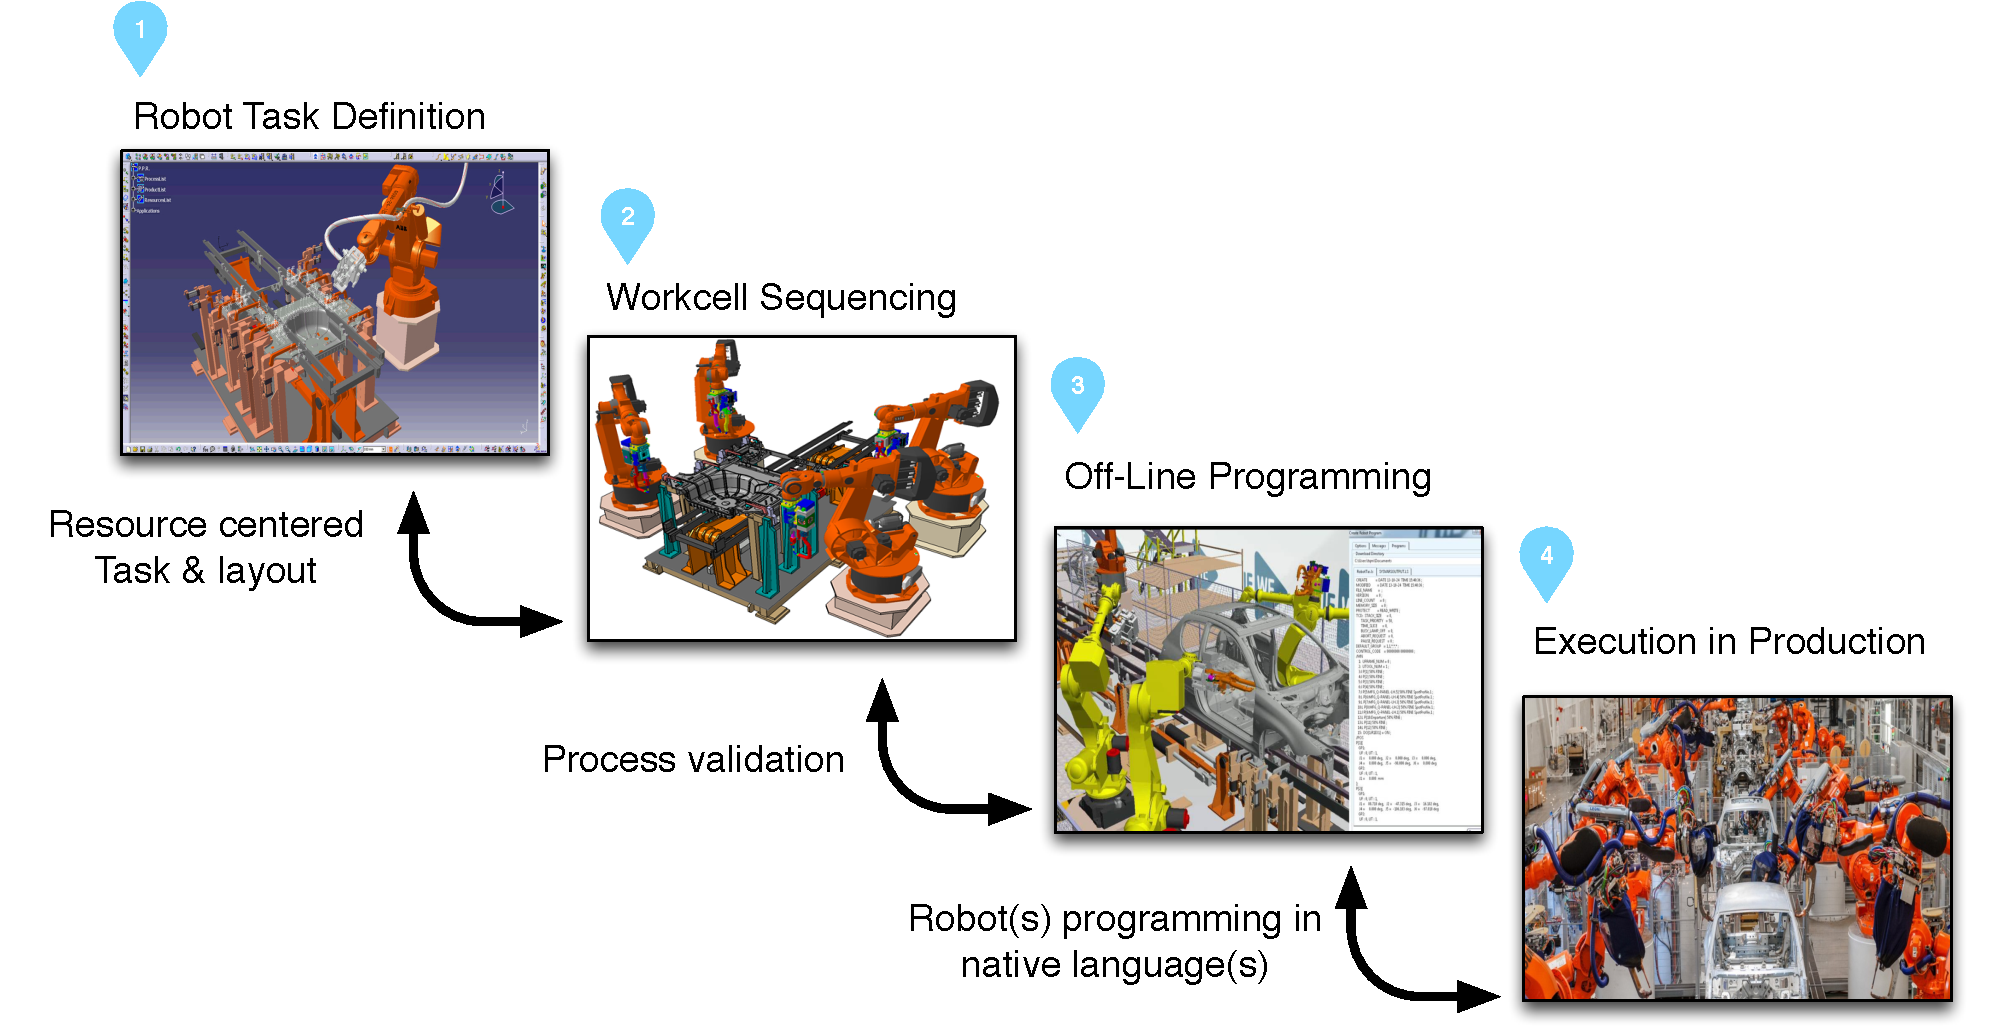
\includegraphics[width=\linewidth]{figures/manual-programming}
	\caption{Classical robot programming process}
	\label{fig:Classical robot programming process}
\end{figure}

In the past few decades, different robot programming techniques have been developed. 
There are many ways to divide robot programming systems. 
\cite{lozano1983robot} divided them into three categories: 
\begin{itemize}
	\item Guiding systems, where the robot's joint positions were sequentially recorded,
	\item Robot-level systems, where a programming language was used,
	\item Task-level systems, where the task goal (e.g. object positions) needed to be specified.
\end{itemize}
However, the range of programming systems was very limited at that time and examined only industrial robot programming systems.
Instead, \cite{Biggs2003} divided them into two main categories, distinguishing systems for users and for programmers (\fig{fig:RobotProgrammingSystems}):

\begin{itemize}
  \item {\textbf{Manual programming}, where the user can directly control the robot's execution code, using a text-based or a graphical system.}
  \item {\textbf{Automatic programming}, where the user does not need to write explicit code and the robot learns using a learning system, programming by demonstration, or an instructive system.}
\end{itemize}
% - also mention software architectures which are important for any robot programming systems

 \begin{figure}[ht]
 \centering
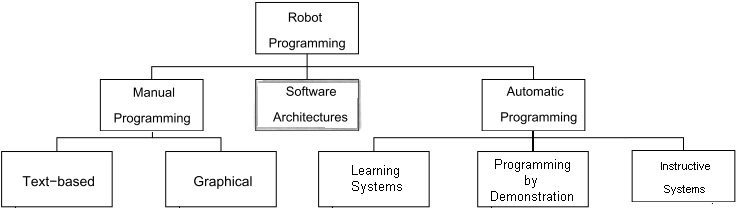
\includegraphics[width=\linewidth]{figures/Biggs2003-RobotProgramming-short}
 \caption{Robot programming categories to distinguish systems for users and programmers. (\cite{Biggs2003})}
 \label{fig:RobotProgrammingSystems}
\end{figure} 

Inspired by \cite{Biggs2003}, \fig{fig:RobotProgrammingOverview} gives an overview of robot programming techniques that have been applied in recent research.
Even though many state of the art systems use a combination of techniques, such as PbD for Reinforcement Learning (\cite{hester2017learning}), it makes sense to differentiate them by their key attributes.
From an end-user programming perspective, it is useful to assign different levels of teacher involvement in the programming process and an estimation of the programming time required.
In the following sections we will give a brief overview of the different programming systems.

%\begin{table}[ht]
%\begin{center}
%\begin{tabular}{r|c|c}
%Programming Techniques & by Exploration \newline (unguided) & by Demonstration \newline (guided)\\ \hline
%Classification & \checkmark & \checkmark \cite{saunders2006teaching,hovland1996skill,rybski1999interactive} \\
%Regression & \checkmark & \checkmark \cite{atkeson1997locally,pomerleau1991efficient} \\
%Reinforcement Learning & \checkmark & \checkmark (System models) \cite{atkeson1997robot,smart2002effective,abbeel2004apprenticeship}.\\
% Plans & \checkmark & \checkmark \cite{kuniyoshi1994learning,ekvall2008robot} \\
% \hline
%Human-Robot Interaction & & \\ \hline
% touch & \checkmark (learning by poking) & \checkmark \\
% vision & \checkmark & \checkmark \\ 
% voice & n/a & \checkmark (instructive, create sequence by voice) \\
%\end{tabular}
%\end{center}
%\label{tab:Programming Overview}
%\end{table}

\begin{figure}[!h]
	\centering
	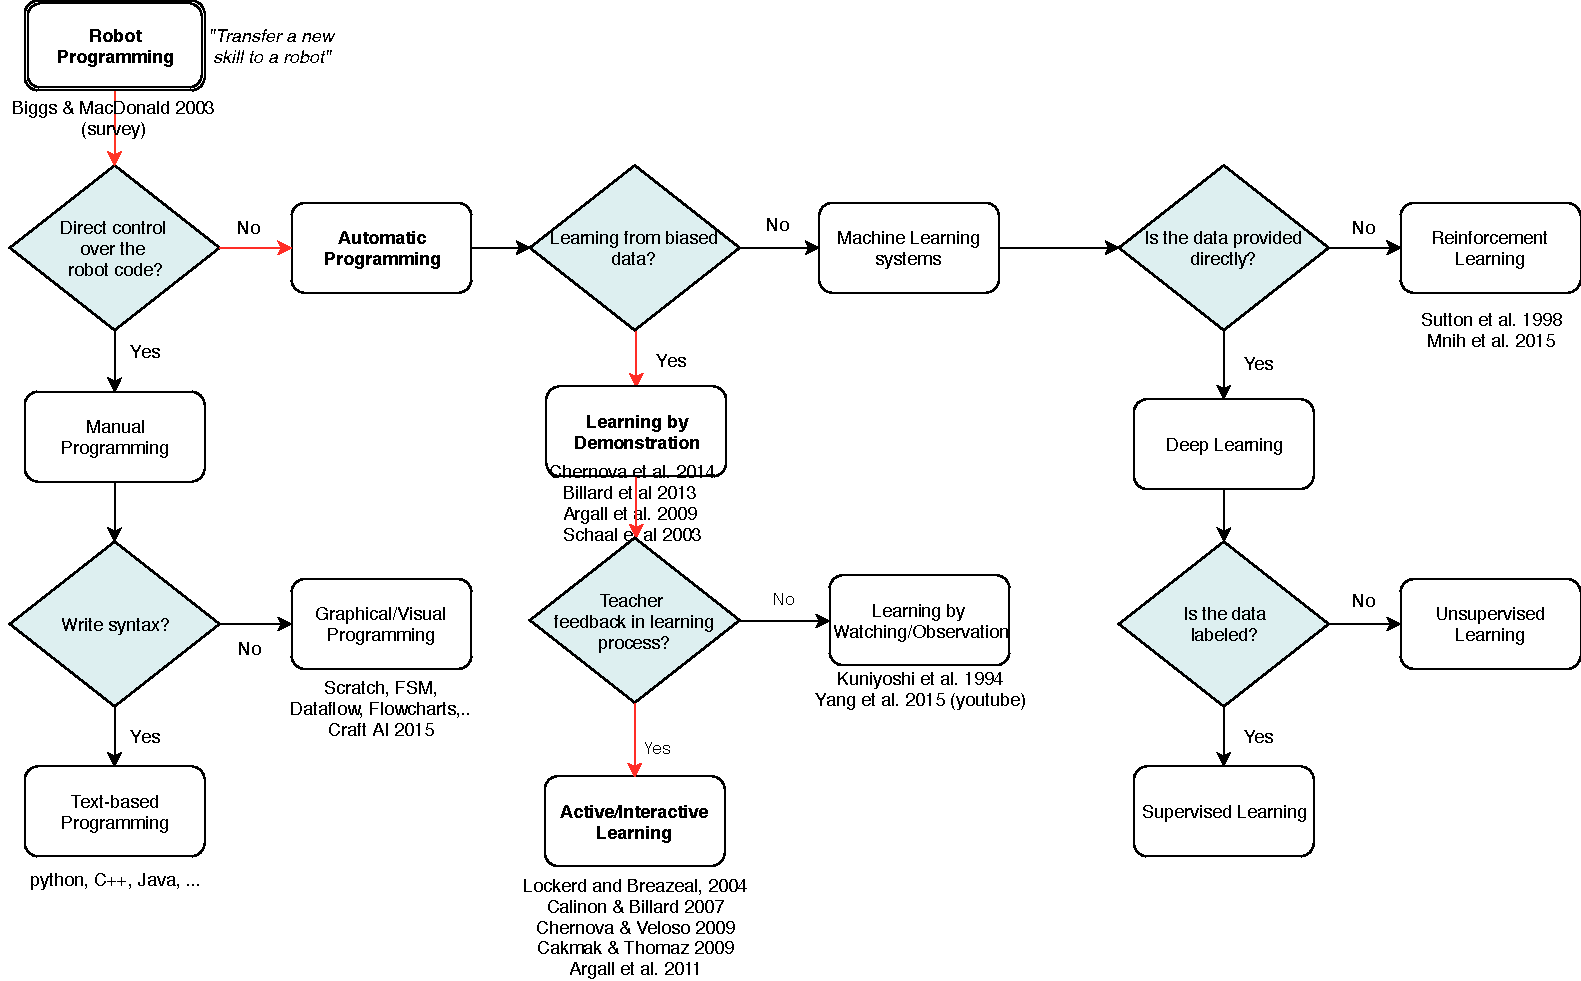
\includegraphics[width=0.87\linewidth]{figures/RobotProgrammingOverview.pdf}
	\caption{Overview of Robot Programming methods.}
	\label{fig:RobotProgrammingOverview}
\end{figure} 

\section{Manual Programming Systems}\label{subsec:Manual Programming Systems}
In manual programming systems users must create the robot program by hand, either using a text-based or a graphical (or icon-based) interface.
While the user has direct control over the robot code, it requires expert knowledge in a programming language and a good understanding of the program flow.
There exist a variety of tools to make programming, as well as testing and debugging easier, such as IDEs, spreadsheets, macros, etc.

There are two types of manual programming: text-based programming, where the code is written manually in a chosen programming language (python, C++, java, etc.) and graphical programming, where the code structure is created with the help of a graphical interface (e.g. Scratch (Majed 2014, Lamb \& Johnson 2011, Schorow 2007), Flowcharts, etc.). 

\subsection{Text-based Systems}\label{sssec:Text-based Systems}
Text-based systems are one of the most common methods and use a traditional programming language approach. 
Depending on the type of language used, the user performs programming in the following languages:
\begin{itemize}
	\item controller-specific: robot-specific machine language consisting of simple commands ({KUKA, ABB})
	\item generic procedural: multi-purpose language (e.g. C++) that has been extended with classes to provide simple access to common robot specific functions ({Lego, etc.})
	\item behaviour-based: specify how the robot should react to different conditions (e.g. Haskell)
\end{itemize}
There has been a the trend to move from low-level command-based languages towards more intelligent programming systems with high-level languages that provide more support to the user and  reduces the programming workload.
However, text-based systems still require trained users with programming knowledge and are more likely to be used by robot developers than end-users.


\begin{figure}[h]
	\centering
	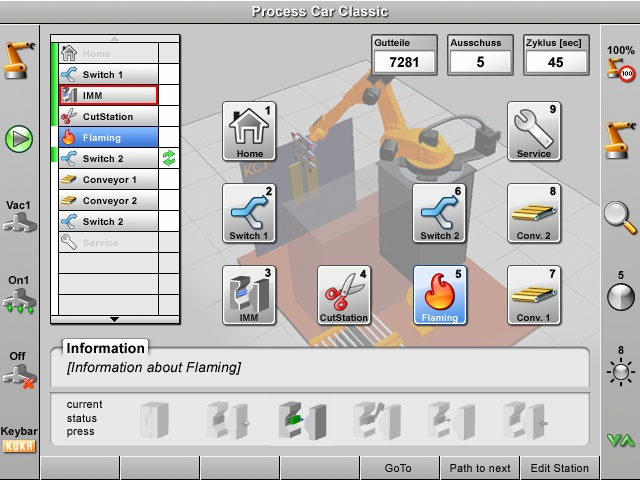
\includegraphics[width=0.8\linewidth]{figures/kuka.jpg}
	\caption{KUKA Robotics graphical user interface (\cite{kuka2006})}
	\label{fig:Kuka}
\end{figure} 

%\todo{Add KUKA interface, lego mindstorms screenshot}

\subsection{Graphical Systems}\label{sssec:Graphical systems}
Graphical (or icon-based) systems use a graph, flow-chart or diagram view where users manually specify actions and program flow (\fig{fig:Kuka}).
The graphical icons correspond directly to the program statements.
They are typically easy to use and generally used for robot applications rather than system programming. 
\cite{lego2003} and \cite{bischoff2002morpha} produced graphical systems using a flow-chart approach, where the robot's behaviour can be configured by arranging low-level actions in a sequence.
%\todo{Add examples of graphical systems}


\section{Automatic Programming Systems}\label{subsec:Automatic Programming Systems}
Automatic programming relates to robots that have the capability to learn from new data.
Unlike manual programming, the user does not need to write explicit robot code and does not have direct control over the code as its behaviour is generated from information entered into the system.
\cite{Biggs2003} divided automatic programming systems between \textit{guided}, where the robot learns with human intervention (e.g. Programming by Demonstration), and \textit{unguided}, where the robot learns by exploration (e.g. Neural Networks, Reinforcement Learning).
Furthermore, the authors mention instructive systems which provides high-level control over underlying pre-programmed capabilities.

\subsection{Learning Systems}\label{sssec:Learning Systems}
Learning systems use inductive inference to create a program by taking examples provided by the user or from self-exploration of the robot. 
The goal of these machine learning (ML) systems is to construct programs that allow the robot to automatically improve its performance with increasing amounts of data. 

Even though ML algorithms have been around since the 1980s, it has only become popular in the past few decades. 
The rise of the internet led to big data, improved knowledge sharing and advances in techniques to process and store data efficiently.
Developments in various research areas such as computer vision have impacted the field of robotics.
In particular, big data and advances in techniques to process and store data efficiently has lead to a wave of new ML techniques. 
Recent applications\footnote{http://techemergence.com/machine-learning-in-robotics/} of ML in robotics include research areas such as computer vision (or ``robot vision'') for the identification and sorting of objects (\cite{stager2013computer}) and imitation learning to learn action plans from watching unconstrained videos (\cite{Yang2015}).

Deep learning systems generally use neural networks (NN) with different architectures which require a large amounts of data to learn the desired behaviour.
\cite{billard2001robust} used NN to learn the motion of a human arm in 3D.
A full review of approaches and techniques in deep learning (\cite{schmidhuber2015deep}) is beyond the scope of this thesis.

%\cite{Kreuziger1992} analysed the application of ML in robotics (\fig{fig:MLvsRobotics}) and identified a large gap between these two research areas.
%\begin{figure}[h]
%	\centering
%	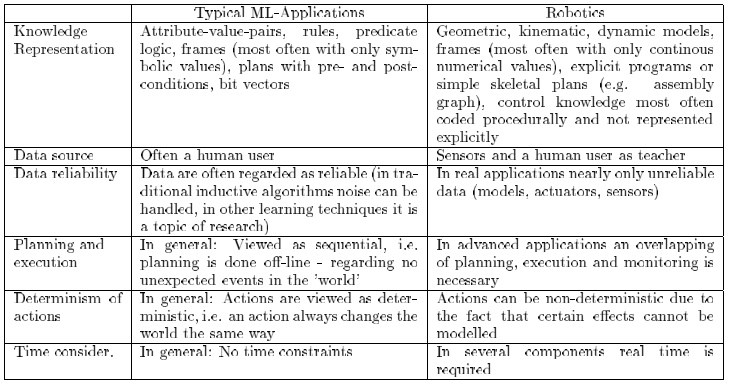
\includegraphics[width=\linewidth]{figures/Kreuziger1992-Comparison ML Robotics}
%	\caption{Comparison on Machine Learning applications vs. Robotics. \cite{Kreuziger1992}}
%	\label{fig:MLvsRobotics}
%\end{figure} 

\subsubsection{Reinforcement Learning}
Rreinforcement learning (RL) (\cite{sutton1998reinforcement,kaelbling1996reinforcement,gosavi2009reinforcement}) requires a reward function which needs to be specified by a domain expert.
There are two main classes of RL approaches, namely model-based (\cite{polydoros2017survey}) and model-free (\cite{kober2013reinforcement}) methods, differentiating between whether a model of the interactions between the robot and the environment is used, or whether it learns from samples.
While model-based methods converge faster to the optimal solution, an accurate model is not always available and can impact the learning process.
Model-free methods require the robot to learn from samples, resulting in a slow convergence to the optimal solution.
cite{kober2013reinforcement} provides a survey of work in RL to generate behaviour for robots and highlights the main challenges that are faced.
To accelerate the learning and reduce the amount of exploration required, work has been done to include teacher demonstrations with RL solutions (\cite{martinez2017relational,hester2017learning}).
In real world scenarios robots require teacher input to learn behaviours efficiently. 
%\todo{Similar to our work: \cite{martinez2017relational}}

The problem with RL solutions is that reward functions are difficult to specify.
Inverse reinforcement learning (\cite{abbeel2011inverse}) is a supervised RL mode where the learner tries to acquire the reward function from demonstrated behaviours.
This is can also be considered a learning from demonstration approach.

\subsection{Programming by Demonstration}
Programming by demonstration (PbD) (\cite{billard2008robot}), also known as Learning from Demonstration, describes various techniques the robot learns new behaviours from teacher demonstrations. 
There are different ways for a teacher to provide demonstration data (\sect{subsec:Gathering demonstrations}), depending on the amount of data provided at a time (incremental vs. batch learning) and the different interaction modalities (touch, vision, gestures, voice) to transfer the data to the robot. 
The robot derives a policy in various ways (\sect{subsec:Deriving a policy}). 

PbD systems have been used in the industry for creating assembly programs. 
In recent years there has been significant work in PbD to move from pure imitation to intelligent systems that learn flexible task executions. 
PbD systems may learn task descriptions from interpreted data to adapt the learned task to changing environments.

\subsection{Instructive Systems}%\todo{Delete or Move}
Instructive systems use gesture or voice recognition to command robots to carry out tasks.
These tasks typically consist of actions that they have already been trained or programmed to do. 
Gestures can be used to direct the attention of the robot for indicating objects in a scene to which the instructions apply. 
Natural language is the most intuitive way for humans to communicate instructions but may need some form of clarification and learning system in order to work efficiently. 
A multi-modal communication including information from vision, gesture and voice sources can be used to clarify instructions to the robot, for example mentioning ``that table" and gesturing the relevant object.
Instructive systems are useful for providing a high-level control but rely on underlying trained abilities which need to be implemented using other programming systems such as manual programming or PbD.


\section{Robot Programming in Industrial Environments}\label{subsec:RP in Industrial Enviroments}
The deployment of robots in industrial environments introduces additional constraints to the robot programming process, such as limited resources, time constraints, limited programming expertise, product-specific tasks.
\cite{pan2012recent} give an overview of three main robot programming methods for industrial robots: offline programming, online programming, and using Augmented Reality. 

\subsection{Offline Programming}\label{sssec:Offline Programming}
Offline Programming (OLP) is based on 3D CAD data that models the complete robot work cell and lets the user fine-tune the properties of the robot's movements before generating a program that can be downloaded to the robot. 
It is more efficient when programming complex systems with large volumes and more reliable compared to online programming. 
As it requires a great amount of programming effort and a long delivery time, it requires high programming overhead and is not efficient for the development of smaller product volumes or customised software.

Robot designers and users have developed computational platforms for OLP systems in form of packages that allow secondary development for specific applications. 
These OLP packages simulate not only robot trajectories and assembly tasks, but can also model interactions of several manufacturing processes, resources and product maintenance issues. 
Almost every robot manufacturer has its own OLP software. 
There exist also generic OLP software that are more flexible for hardware from different manufacturers.

Current OLP systems do not provide functions for the complete OLP process but include steps that need to be created manually. 
Due to the high costs of OLP systems, their use is not cost-efficient for small to medium-sized enterprises.

\subsection{Online Programming}\label{sssec:Online Programming}
In online programming methods the robot program commands the robot to move through a recorded sequence of end-effector postures which form a complete task. 
The postures are recorded using the teach pendant to manually move the end-effector to the desired position and orientation of the task. 
Due to its simplicity, intuitiveness, and low programming skill requirement, this method is widely used. 
However, it is only suitable for programming applications with uncomplicated processes and work pieces with simple geometry. 
Once the program has been generated, it is difficult to make further amendments.

\subsection{Augmented Reality}\label{sssec:Augmented Reality}
The use of augmented reality (AR) is a revolutionary concept where computer-generated 3D objects are blended onto a real world scene to enhance the user's interaction with the real world (\cite{pettersen2003augmented}). 
Robot programming using AR allows offline programming to be performed without the need to model the workpiece in the virtual environment (\cite{pan2012recent}). 
It can eliminate technical difficulties faced by OLP techniques such as the calibration between the virtual and the real world.
